\documentclass[11pt]{article}

% Allows Hyperlinks
\usepackage{hyperref}

% Sets more normal margins
\usepackage{fullpage}

% Use biblatex
\usepackage[style=authoryear, natbib=true]{biblatex}
\bibliography{refs}

% Use Verbatim for showing commands 
\usepackage{verbatim}

% Get Array Package for Tables and Graphic Alignment
\usepackage{array}

% Allow Importing of Graphics
\usepackage{graphicx}

% Allow for Double Space
\usepackage{setspace}

% Align Equations
\usepackage{amsmath}

\begin{document} 

\title{LaTeX Basics}
\date{}
\author{\textbf{Ben O. Smith\footnote{\href{mailto:ben@bensresearch.com}{ben@bensresearch.com}}} \\
School of Economic Sciences \\
Washington State University}
\maketitle 

\section*{Learning Objectives}

By the end of this document you will learn:

\begin{enumerate}
	\item How to setup a basic LaTeX document
	\item Include the appropriate packages in the header
	\item Interact with sections and separate your project into smaller files
	\item Cite sources and create a reference section
	\item Include equations and figures in your document
\end{enumerate}

\doublespace
\section{Structure of a LaTeX Document}

A LaTeX document is a tree-like structure where nodes (or environments) can have sub-nodes.  Let's start with an extremely basic LaTeX document:

\begin{quote}
	\begin{verbatim}
		\documentclass[11pt]{article}
		
		\begin{document} 
		
		\section{Introduction}
		Lorem ipsum dolor sit amet, consectetur adipiscing elit...
		
		\subsection{Why this is important}
		Suspendisse eget urna urna, ut pharetra odio....
		
		\section{Conclusion}
		In sed sem quis leo convallis tempor....		
		\end{document}
	\end{verbatim}
\end{quote}

\subsection{The Header and Packages}

The area between:

\begin{quote}
	\begin{verbatim}
		\documentclass[11pt]{article}
	\end{verbatim}
\end{quote}

And 

\begin{quote}
	\begin{verbatim}
		\begin{document} 
	\end{verbatim}
\end{quote}

Is called the header.  This is the area where we import packages (which adds a set of functions to LaTeX) and set options or settings.  For instance, the default margins (in my opinion) are strange.  So, I'm going to add a package that sets the margins to more traditional settings:

\begin{quote}
	\begin{verbatim}
		\usepackage{fullpage}
	\end{verbatim}
\end{quote}

Adding a package is just that easy.  ``usepackage" takes the following general form:

\begin{quote}
	\begin{verbatim}
		\usepackage[options]{PackageName}
	\end{verbatim}
\end{quote}

Options can often be omitted, which will result in the default behavior of the package. 

\subsection{The Document and Your Content}

The area between:

\begin{quote}
	\begin{verbatim}
		\begin{document} 
	\end{verbatim}
\end{quote}

And

\begin{quote}
	\begin{verbatim}
		\end{document} 
	\end{verbatim}
\end{quote}

Is where you write your content.  Note the use of $\backslash begin\{document\}$ and $\backslash end\{document\}$.  This means that anything between ``begin" and ``end" is part of the document node.  There might be equations, tables or other ``environments" that you start and stop with $\backslash begin\{\cdot\}$ and $\backslash end\{\cdot\}$, but because you haven't ended the document, they are sub-nodes of the document.

\subsubsection{Sections}

$\backslash section\{Section~Title\}$ starts a section.  A section can have a subsection by using the command $\backslash subsection\{Subsection~Title\}$.  You can think of subsections as sub-nodes of the section.  In both the case of sections and subsections, the nodes are numbered.  So, the first section of your document will take the number ``1", while the first subsection of a section would take the the number ``[section number].1".  Section numbering can be suppressed by using a ``*" like so: $\backslash section^*\{Section~Title\}$.  Most, but not all, environments that auto-number suppress their numbering when you include a ``*".

Another set of commands you might want to use is $\backslash label\{\cdot\}$ and $\backslash ref\{\cdot\}$.  Nodes and sub-nodes in the document can generally be labeled so you can reference them without worrying about the auto-numbering changing.  For instance I might label the introduction like so:

\begin{quote}
	\begin{verbatim}
		\section{Introduction}
		\label{sec:introduction} 
	\end{verbatim}
\end{quote}

Then later in the document, I could write:

\begin{quote}
	\begin{verbatim}
		As discussed in section \ref{sec:introduction} ...
	\end{verbatim}
\end{quote}

No matter how I rearrange the document, the number in that sentence will be correct.

\subsubsection{Using \textbackslash input}

One of the best features of LaTeX is the ability to break a long document into smaller files.  This is accomplished by using the $\backslash input$ command.  For instance, if I wanted to have a separate file for each section, my document might look like this:

\begin{quote}
	\begin{verbatim}
		\documentclass[11pt]{article}
		
		\begin{document} 
		
		\input{Introduction}
		\input{Conclusion}
			
		\end{document}
	\end{verbatim}
\end{quote}

Where I have two files in the same  directory (folder) as your main LaTeX document: ``Introduction.tex" and ``Conclusion.tex".  Not only does this keep your documents clean, it makes it easy to reorganize without having to copy and paste large chunks of text.
\section{Equations}

Equations are a built-in feature to LaTeX, no package is needed. Equations can be included in a paragraph of text by using the ``\$", or as an environment/node by using the $\backslash begin\{equation\}$ and $\backslash end\{equation\}$ commands.  I might write something like the following in a paragraph:

\begin{quote}
	\begin{verbatim}
		$R = R_{cd}g^{cd}$ is the curvature scale in Einstein's field equations...
	\end{verbatim}
\end{quote}


To insert an equation into your text as an environment, you need only write:

\begin{quote}
	\begin{verbatim}
		\begin{equation}
			R = R_{cd}g^{cd}
		\end{equation}
	\end{verbatim}
\end{quote}

Like sections, equation environments are auto-numbered by default, but this can be suppressed by including a ``*" like so:

\begin{quote}
	\begin{verbatim}
		\begin{equation*}
			R = R_{cd}g^{cd}
		\end{equation*}
	\end{verbatim}
\end{quote}

Like aligned enviroments (section \ref{eqwithalign}), using \emph{equation*} requires loading the \emph{amsmath} package.  I cover loading that package in section \ref{eqwithalign}.

Further, you can reference equations by using $\backslash label\{\cdot\}$ and $\backslash ref\{\cdot\}$.  For instance, I might do the following:

\begin{quote}
	\begin{verbatim}
		\begin{equation}
			\label{eq:tensor}	
			R = R_{cd}g^{cd}
		\end{equation}
		
		According to equation \ref{eq:tensor} ...
	\end{verbatim}
\end{quote}

And know that my equation number will always be correct.

\subsection{Equations with Aligned}
\label{eqwithalign}

One of the problems that you might run into is when your equation is too long for a single line.  The way to solve this problem is to add an aligned environment inside of your equation environment.  However, to create an aligned environment inside of of an equation, you need to load an additional package:

\begin{quote}
	\begin{verbatim}
		\usepackage{amsmath}
	\end{verbatim}
\end{quote}

Now, you could do something like this:

\begin{quote}
	\begin{verbatim}
		\begin{equation}
			\begin{aligned}
	  			\pi_t(\cdot) &= q_p(\cdot)P_p - C_p q_p(\cdot) - F - C_s q_p(\cdot) \\
	  			& - C_s q_p(\cdot) \int\limits_0^w{e^{-rt}f(t)S(t)dt} \\
	  			& + (q_s(\cdot)P_s - C_sq_s(\cdot))\int\limits_w^T{e^{-rt}f(t)S(t)dt}
	 		\end{aligned}
		\end{equation}
	\end{verbatim}
\end{quote}

Which produces:

\begin{equation}
	\begin{aligned}
		\pi_t(\cdot) &= q_p(\cdot)P_p - C_p q_p(\cdot) - F - C_s q_p(\cdot) \\
	  	& - C_s q_p(\cdot) \int\limits_0^w{e^{-rt}f(t)S(t)dt} \\
	  	& + (q_s(\cdot)P_s - C_sq_s(\cdot))\int\limits_w^T{e^{-rt}f(t)S(t)dt}
	 \end{aligned}
\end{equation}

Notice, that the equation is aligned to the ``\&" for each line and you use ``\textbackslash \textbackslash" to indicate a new line.


\section{References and Citations}

References in LaTeX have two main components, a ``.bib" file and a package that allows you to cite the articles in your text.  Then you simply place the bibliography at the end of your document.  

\subsection{The ``Bib" File}

Here is an example bib file with an entry for \emph{The Wealth of Nations}: 

\begin{quote}
	\verbatiminput{refs.bib}
\end{quote}

So, you might already have a reference manager.  If you don't, I'd recommend \href{http://www.mekentosj.com/papers/}{Papers}\footnote{\href{http://www.mekentosj.com/papers/}{http:/\slash www.mekentosj.com\slash papers}} if you want to sync your PDFs to multiple devices (e.g. computers+iPad) or \href{http://jabref.sourceforge.net}{JabRef}\footnote{\href{http://jabref.sourceforge.net}{http:/\slash jabref.sourceforge.net}} which has the advantage of being free.  Regardless, \emph{any good} reference manager will export a bib file -- you do not have to make this by hand.  

\subsection{Citations with NatBib or Biblatex}

Now, there are two reasonable choices of packages for citations: natbib and biblatex. Biblatex is the new hotness, it has a bunch of features (many of which I'm not sure why anyone would use) and it is under active development. Natbib is old, and is missing many of the new fancy features in biblatex.  However, because of its age, there is a lot of style files (``*.bst" files) prebuilt.  Here is some natbib citation commands:

\begin{table}[h]
\centering
	\begin{tabular}{m{8cm}l}
		Command       & Output \tabularnewline \hline
 		 \begin{verbatim}\citet{Smith:1776uz}\end{verbatim}
 		& \citet{Smith:1776uz}      \tabularnewline 
 		\begin{verbatim}\citep{Smith:1776uz}\end{verbatim}
 		& \citep{Smith:1776uz}			\tabularnewline
 		\begin{verbatim}\citet[See Ch. 2]{Smith:1776uz}\end{verbatim}
 		& \citet[See Ch. 2]{Smith:1776uz}     \tabularnewline
 	\end{tabular}
\end{table}

In a sentince I might write:

\begin{quote}
	\begin{verbatim}
		Economist know that mercantilism is a failed idea \citep{Smith:1776uz}.
	\end{verbatim}
\end{quote}

To use natbib, you need to include the following in your header:

\begin{quote}
	\begin{verbatim}
		\usepackage{natbib}
	\end{verbatim}
\end{quote}

And, in the content of your document, where you want your bibliography:

\begin{quote}
	\begin{verbatim}
		\bibliographystyle{apalike}
		\bibliography{BibFile}
	\end{verbatim}
\end{quote}

Where ``apalike" is the name of your bibliography style (apalike is one of the built-in styles) and ``BibFile" is the name of your ``.bib" file.
 
What about biblatex? In your header include:

\begin{quote}
	\begin{verbatim}
		\usepackage[style=authoryear]{biblatex}
		\bibliography{BibFile}
	\end{verbatim}
\end{quote}

And simply place:

\begin{quote}
	\begin{verbatim}
		\printbibliography[title=Bibliography]
	\end{verbatim}
\end{quote}

Where you want your bibliography.  Biblatex actually has its own commands for textual and parenthetical citations (i.e. $\backslash textcite$ and $\backslash parencite$) and an amazing number of other commands.  The problem is that biblatex is new and a lot of people don't use it.  So, what I do is modify my ``usepackage" options so that I use biblatex but with natbib citation commands:

\begin{quote}
	\begin{verbatim}
		\usepackage[style=authoryear, natbib=true]{biblatex}
		\bibliography{refs}
	\end{verbatim}
\end{quote}

That way I can quickly switch back to natbib by just modifying my header lines (and not every citation), but I still get the benefits of using a system that is under active development.
\section{Images and Figures}

Images can be included in LaTeX documents fairly easily.  However, you must include a package first in your header:

\begin{quote}
	\begin{verbatim}
		\usepackage{graphicx}
	\end{verbatim}
\end{quote}

Then, in your text where you want the graphic, put:
\begin{quote}
	\begin{verbatim}
		\includegraphics[width=5in]{graphics/number_of_firms.eps}
	\end{verbatim}
\end{quote}

The type of graphics you can include depends on your typesetter, but there are two big ones: PDF and EPS.  In most cases, if what you want to include is a graph or diagram, you should be using EPS.  

Sometimes your graphic will be a figure that you want to reference.  In that case, you can wrap the graphic in a figure:

\begin{quote}
	\begin{verbatim}
		\begin{figure}[hbt]
  			\centering
  			\includegraphics[width=5in]{graphics/number_of_firms.eps}
  			\caption{As the number of firms increase...}
  			\label{fig:firms}
  		\end{figure}
	\end{verbatim}
\end{quote}

Which produces this:

\begin{figure}[hbt]
	\centering
  	\includegraphics[width=5in]{graphics/number_of_firms.eps}
  	\caption{As the number of firms increase...}
  	\label{fig:firms}
\end{figure}

The figure options ``[hbt]" tell LaTeX what part of the page the figure can appear (in this case: ``here" - h, ``bottom" - b or ``top" - t).  I can also reference this figure by using \emph{\textbackslash ref\{fig:firms\}}.

\section{LaTeX Resources}

\subsection{LaTeX Packages}
\label{latexpackages}

\begin{itemize}
\item \href{http://www.miktex.org}{LaTeX for Windows}\footnote{\href{http://www.miktex.org}{http:/\slash www.miktex.org}}

\item \href{http://www.tug.org/mactex/}{LaTeX for Mac}\footnote{\href{http://www.tug.org/mactex/}{http:/\slash www.tug.org\slash mactex\slash }}

\item \href{http://www.tug.org/texlive/}{LaTeX for Linux}\footnote{\href{http://www.tug.org/texlive/}{http:/\slash www.tug.org\slash texlive\slash }}

\item \href{http://www.macports.org}{MacPorts}\footnote{\href{http://www.macports.org}{http:/\slash www.macports.org}}

\item \href{http://www.macports.org/ports.php?by=name&substr=texlive}{LaTex Port Files}\footnote{\href{http://www.macports.org/ports.php?by=name&substr=texlive}{http:/\slash www.macports.org\slash ports.php?by=name\&substr=texlive}}

\end{itemize}

\subsection{Tex Editor}
\label{texeditor}

\begin{itemize}
\item \href{http://texpadapp.com}{TexPad}\footnote{\href{http://texpadapp.com}{http:/\slash texpadapp.com}}

\item \href{http://www.texniccenter.org}{TeXnic Center}\footnote{\href{http://www.texniccenter.org}{http:/\slash www.texniccenter.org}}

\end{itemize}

\subsection{Show Pretty Equations}
\label{showprettyequations}

\begin{itemize}
\item \href{http://klatexformula.sourceforge.net}{KLatexFormula}\footnote{\href{http://klatexformula.sourceforge.net}{http:/\slash klatexformula.sourceforge.net}}

\item \href{http://www.chocomoko.com/brisk}{Brisk}\footnote{\href{http://www.chocomoko.com/brisk}{http:/\slash www.chocomoko.com\slash brisk}}

\end{itemize}

\subsection{References}
\label{references}

\begin{itemize}
\item \href{http://en.wikibooks.org/wiki/LaTeX}{LaTeX on WikiBooks}\footnote{\href{http://en.wikibooks.org/wiki/LaTeX}{http:/\slash en.wikibooks.org\slash wiki\slash LaTeX}}
\item \href{http://www.stdout.org/~winston/latex/latexsheet.pdf}{LaTeX Cheat Sheet}\footnote{\href{http://www.stdout.org/~winston/latex/latexsheet.pdf}{http:/\slash www.stdout.org\slash \textasciitilde winston\slash latex\slash latexsheet.pdf}}
\item \href{http://www.tug.org/pracjourn/2007-1/mori/mori.pdf}{Tables in LaTeX 2e}\footnote{\href{http://www.tug.org/pracjourn/2007-1/mori/mori.pdf}{http:/\slash www.tug.org\slash pracjourn\slash 2007-1\slash mori\slash mori.pdf}}

\end{itemize}



\printbibliography[title=Bibliography]
\vspace{\fill}
\noindent $ \begin{array}{l} \href{http://creativecommons.org/licenses/by/3.0/us/}{
\includegraphics[width=0.25in]{graphics/cc.eps}} \end{array} $ Ben Smith, 2012: \href{http://creativecommons.org/licenses/by/3.0/us/}{Licensed under Creative Commons Attribution 3.0}
\end{document}